\chapter{Funkcja celu -- porównanie barwy dźwięku} \label{target_function_chapter}

Aby stopniowo dostosować graf przetwarzania sygnałów zaimplementowany 
w rozdziale~\ref{dsp_graph_chapter} do imitowania zadanej próbki dźwięku,
należy wykorzystać funkcję celu, która maleje wraz ze wzrostem podobieństwa
barwy dźwięku między próbki zadaną i sygnałem generowanym przez graf. 

\begin{figure}[H]
    \centering
    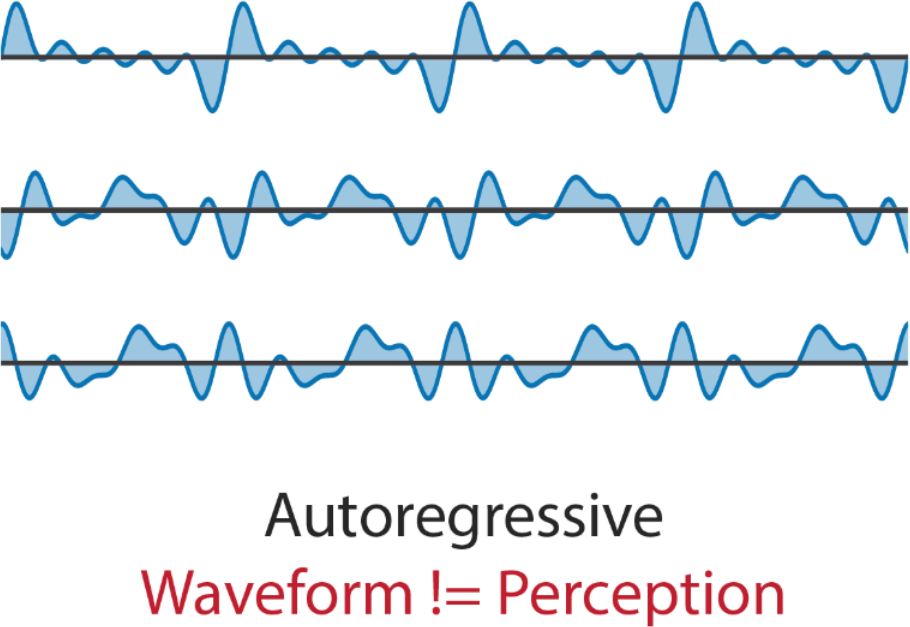
\includegraphics[width=0.5\linewidth]{rys03/d_dsp_example_graph.png}
    \caption{
      Przykład trzech próbek dźwięku, które dla słuchacza brzmią identycznie, mimo
      znacznych różnic w kształcie fali. Źródło obrazka: \cite{engel2020ddsp}.
    }
    \label{fig:waveform_not_equal_to_perception}
\end{figure}

\section{Porównanie barwy dźwięku w literaturze} \label{sec:timbre_comparison_literature_overview}

Żadna z prac przeanalizowanych podczas przeglądu literatury
(\cite{engel2020ddsp}, \cite{ieee_synth_programming}, \cite{ddx7}, \cite{riffusion},
\cite{evolutionary_puredata}, \cite{parallel_evolutionary_optimization_synth_parameters}, \cite{mfcc_dtw})
nie wykorzystuje metod porównywania sygnału osadzonych jedynie w dziedzinie czasu, ponieważ
nie są one skuteczne do porównywania dźwięków pod względem odczuć psychoakustycznych.
Przykład różnych kształtów fali, które z perspektywy słuchacza brzmią jak
taki sam dźwięk zademonstrowano na rysunku~\ref{fig:waveform_not_equal_to_perception}.

Ponieważ porównywanie barwy dźwięku instrumentów muzycznych nie należy do popularnych
tematów badań, podczas przeglądu literatury wykorzystano również badania dotyczące
rozpoznawania głosu, wykorzystujące współczynniki MFCC oraz
\textit{dynamic time warping}~(DTW)~\cite{mfcc_dtw}.

\subsection{Systematyzacja metod z literatury} \label{sec:timbre_comparison_systematisation}

Metody zaczerpięte z literatury wykorzystują różne podejścia do porównywania barwy dźwięku
pomiędzy sygnałami. Podejścia te można usystematyzować za pomocą dwóch cech:

\begin{enumerate}
  \item Rodzaj wykonanej transformacji do dziedziny częstotliwości:
  \begin{itemize}
    \item transformata Fouriera (w różnych konfiguracjach) \cite{riffusion} \cite{ddx7},
    \item MFCC \cite{ieee_synth_programming} \cite{evolutionary_puredata} \cite{mfcc_dtw}.
  \end{itemize}
  \item Dalsze przetwarzanie przetransformowanego sygnału w celu ułatwienia optymalizacji:
    \begin{itemize}
      \item dostosowywanie wagi konkretnych próbek na podstawie metryki określającej siłę sygnału
        (na przykład \textit{root-mean-square}, RMS)
        \cite{parallel_evolutionary_optimization_synth_parameters},
        aby wzmocnić istotność głośniejszych fragmentów dźwięku,
      \item wykorzystanie \textit{dynamic time warping}, aby funkcja celu przyzwalała na
        niedokładności w odwzorowaniu dokładnej dynamiki zmian w charakterystyce spektralnej \cite{mfcc_dtw}.
    \end{itemize}
\end{enumerate}

\subsection{Wybór funkcji celu do przetestowania}

Na podstawie analizy metod z literatury opisanej w rozdziale~\ref{sec:timbre_comparison_systematisation} zostały wybrane wszystkie warianty
funkcji celu wykorzystywane w przeanalizowanej literaturze:

\begin{enumerate}
  \item Różnica w spektrum Fouriera,
  \item Różnica w spektrum Fouriera liczona za pomocą DTW,
  \item Różnica w spektrum Fouriera ważonym za pomocą RMS.
  \item Różnica w MFCC,
  \item Różnica w MFCC liczona za pomocą DTW,
  \item Różnica w MFCC ważonym za pomocą RMS.
\end{enumerate}

\section{Proces testowania funkcji celu}

Funkcje celu zostały przetestowane poprzez wykonwanie
zbioru przekrojów przez uproszczony problem syntezy typu FM.
Testy obejmowały wygenerowanie wartości funkcji celu podczas
modyfikowania pojedynczego parametru w grafie przetwarzania sygnałów
przedstawionym na rysunku~\ref{fig:fm_graph_for_benchmarks}.
Modyfikowane parametry odpowiadają za różne cechy barwy uzyskanego dźwięku:

\begin{itemize}
  \item \texttt{HarmonicMultiplier/input\_scale}:  składowe harmoniczne sygnału,
  \item \texttt{SineOscillator/input\_modulation\_index}: siła składowych harmonicznych,
  \item \texttt{ADSR/input\_attack}: dynamika dźwięku.
\end{itemize}

\begin{figure}[H]
    \centering
    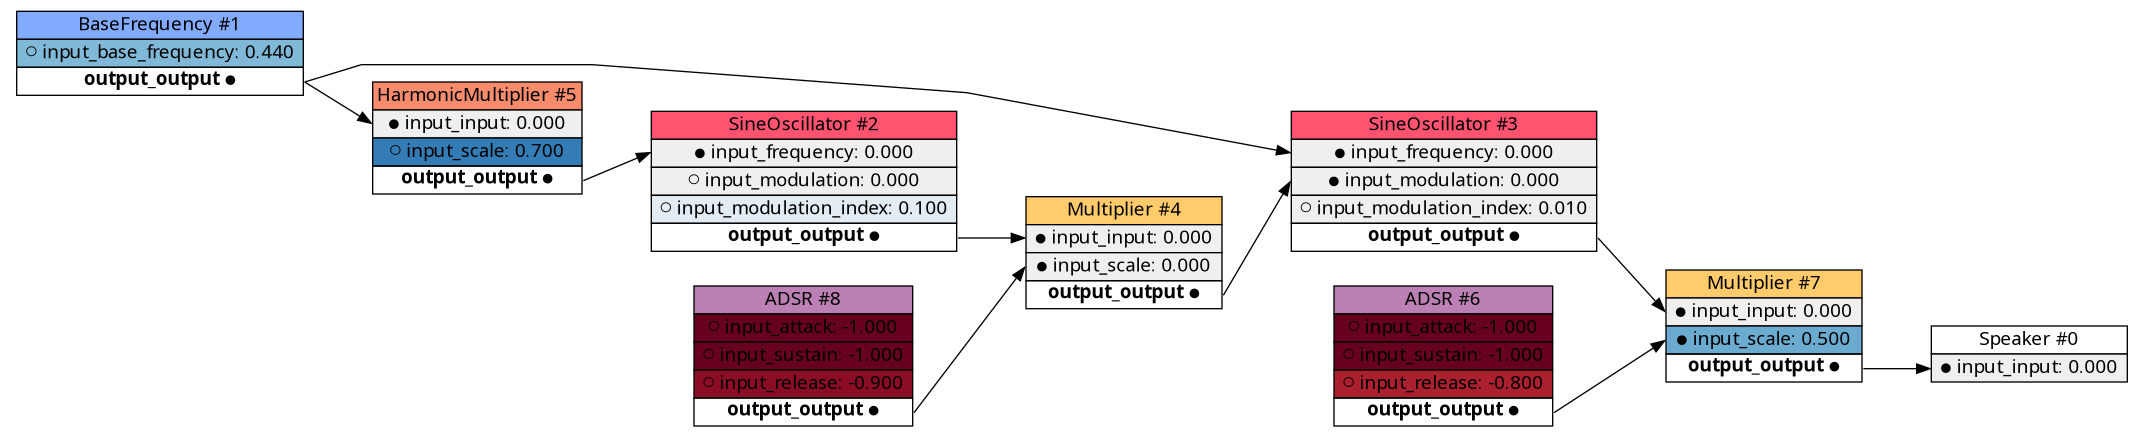
\includegraphics[width=1.0\linewidth]{rys03/fm_graph_for_benchmarks.png}
    \caption{
      Prosty graf syntezy FM, zawierający jeden oscylator służący za sygnał nośny
      i jeden oscylator służący za sygnał modulujący.
    }
    \label{fig:fm_graph_for_benchmarks}
\end{figure}
